\subsection{Configuration of a Location}

Before indoor positioning can be performed, 
we must configure the location in where we want to perform the positioning in. 
For Estimote, this is done using the \texttt{ESTLocationBuilder} as described in \Cref{sec:indoor-positioning:estimote}. 
The location builder is sufficient from a developers perspective, 
but configuring locations in code is likely not intuitive for the target group. 
Instead we propose an alternative way to configure locations.

As a minimum, Estimote must be configured with the walls of a location, 
as the beacons are attached to a wall. 
We propose a smartphone application in which users can draw the walls in their home, 
using the touchscreen of the phone. 
This requires users to measure the length of the walls in their home, 
and then plot it on their smartphone. 
For improved accuracy users can fine tune the length of walls, 
by selecting a wall and entering the length in centimeters.

Having configured the walls of the room, 
the user needs to configure the locations of each beacon. 
The first thing he must do is to install the beacons on the actual walls, 
\ie not the virtual representation of his home.
Using the smartphone application, the user can drag a virtual beacon into the representation of his home, 
and place it on one of the previously configured walls. 
He should do so for each installed beacon.
\todo[author=Simon]{Indsæt evt. reference til testresultater for at addressere mulighed for at mulighed for at indstille beacons, eks. signalstyrke og broadcasting interval.}


The Estimote Indoor SDK must know the MAC address of each positioned beacon, 
in order to do the positioning. 
Using Estimote's regular SDK, \ie not the Indoor SDK, 
signal strengths and MAC addresses for all beacons can be retrieved. 
Based on the signal strengths, 
we can determine which beacon the user is closest to, 
and assign its MAC address to the previously positioned beacon. 
This requires the user to walk along the perimeter of the location when configuring the beacons, 
in order to be closer to the relevant beacon than the rest.

Knowing the layout of the room and the positions of the beacons, 
we can start positioning the user, 
and the only thing left is to configure the location of each actuator, 
in order to determine the relative location of the user and the actuator. 
We can utilize the position of the user when configuring the position of each actuator. 
The user can walk to each actuator he desires to add to the system, 
press a button to add it and for further reference provide some information about the actuator, such as a name.

\Cref{fig:configuration-location:add-room} shows a mock up of software that can be used to configure a location. 
Note that this software was not implemented during the project. 

\Cref{fig:configuration-location:add-room:draw} shows the process of drawing the location. 
The user can use the pencil to draw walls, 
and the erase tool to remove entire walls. 
Tapping on the lengths will present a keyboard, 
allowing the user to adjust the lengths. 
Note that the length of the first wall must be specified manually, 
in order to determine relative lengths when the user draws the following walls.
%Thalley: Giver det mening at sige at vi ikke har implementeret dette? Kunne man ikke nævne det i det næste kapitel?

In \Cref{fig:configuration-location:add-room:beacons} the beacon tool is enabled, 
and the pencil tool and eraser tool are disabled. 
The user should position beacons on the walls, 
by dragging a beacon from the bottom onto a wall.

\Cref{fig:configuration-location:add-room:actuators} shows the user walking around placing actuators. 
Actuators are represented by a circle, 
and two has been placed in the image. 
Recently one was placed at the users current location, 
thus a circle has been put around the user. 
Tapping an actuator lets the user add information about the actuator, such as a name. 
Pressing the done button will save the location.

Locations are created and saved using the \texttt{ESTLocationBuilder}. 
Whenever a location is saved, 
it is stored in the Estimote cloud, 
and is available on all the user's devices. 
In order to authenticate an account with Estimote, 
the user must log into Estimote on \url{cloud.estimote.com}, 
create an application, 
and enter the returned application token into the settings of the smartphone application.

\begin{figure}[!htb]%
    \centering
    \subbottom[Drawing a room]{\label{fig:configuration-location:add-room:draw}
        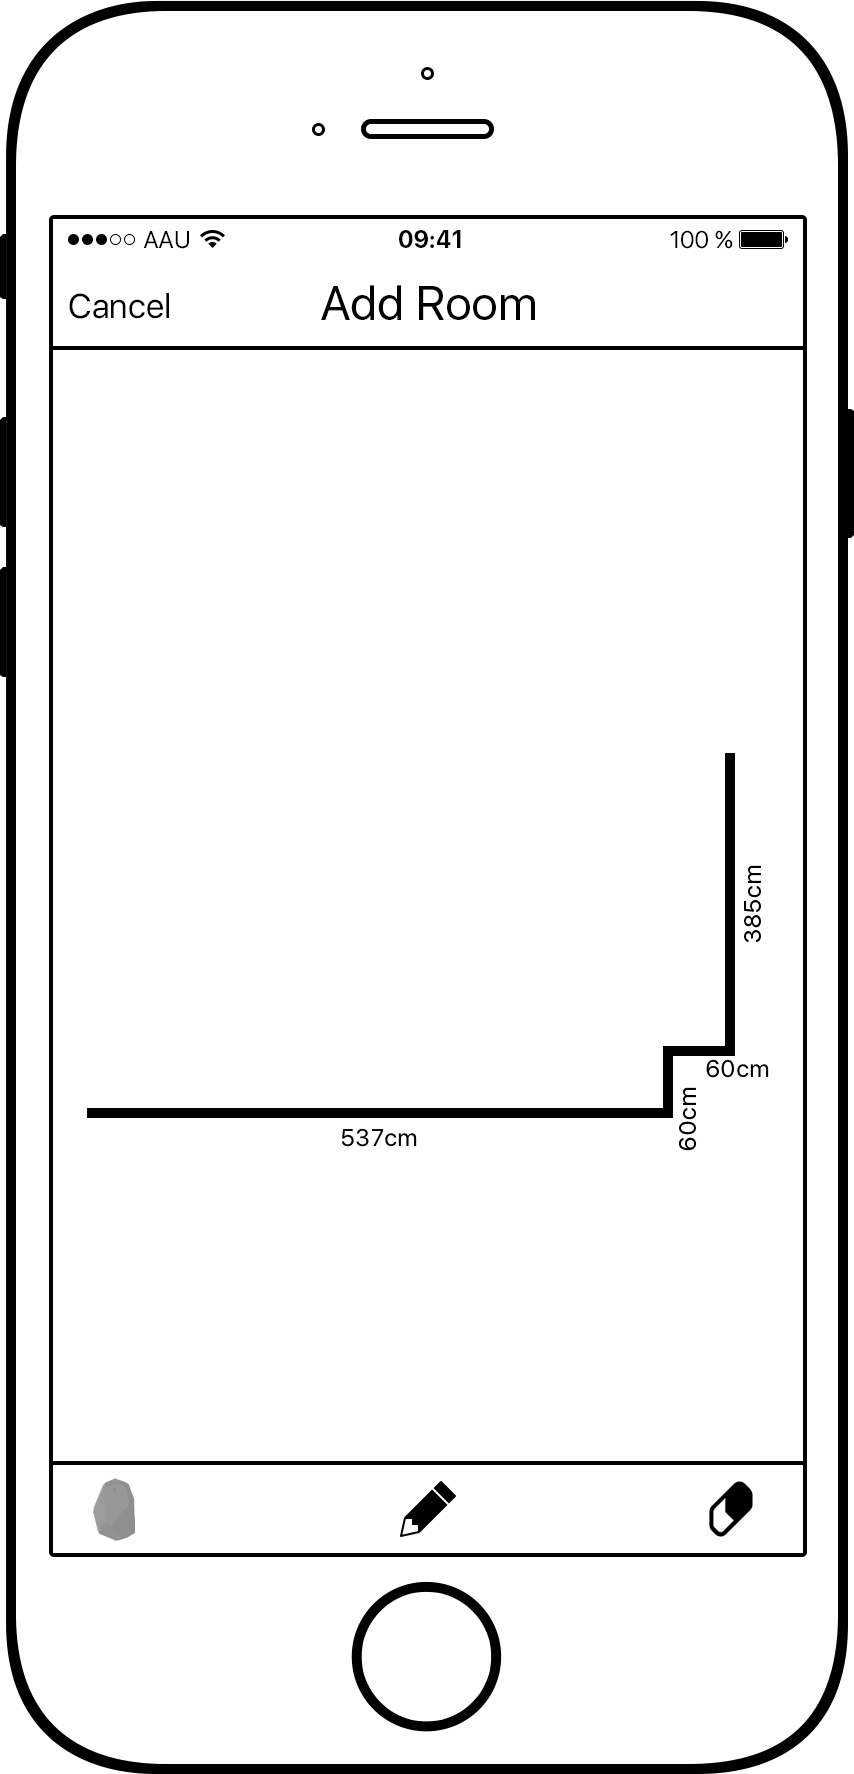
\includegraphics[width=0.3\textwidth]{images/add-room-1}
    }
    \subbottom[Placing beacons]{\label{fig:configuration-location:add-room:beacons}
        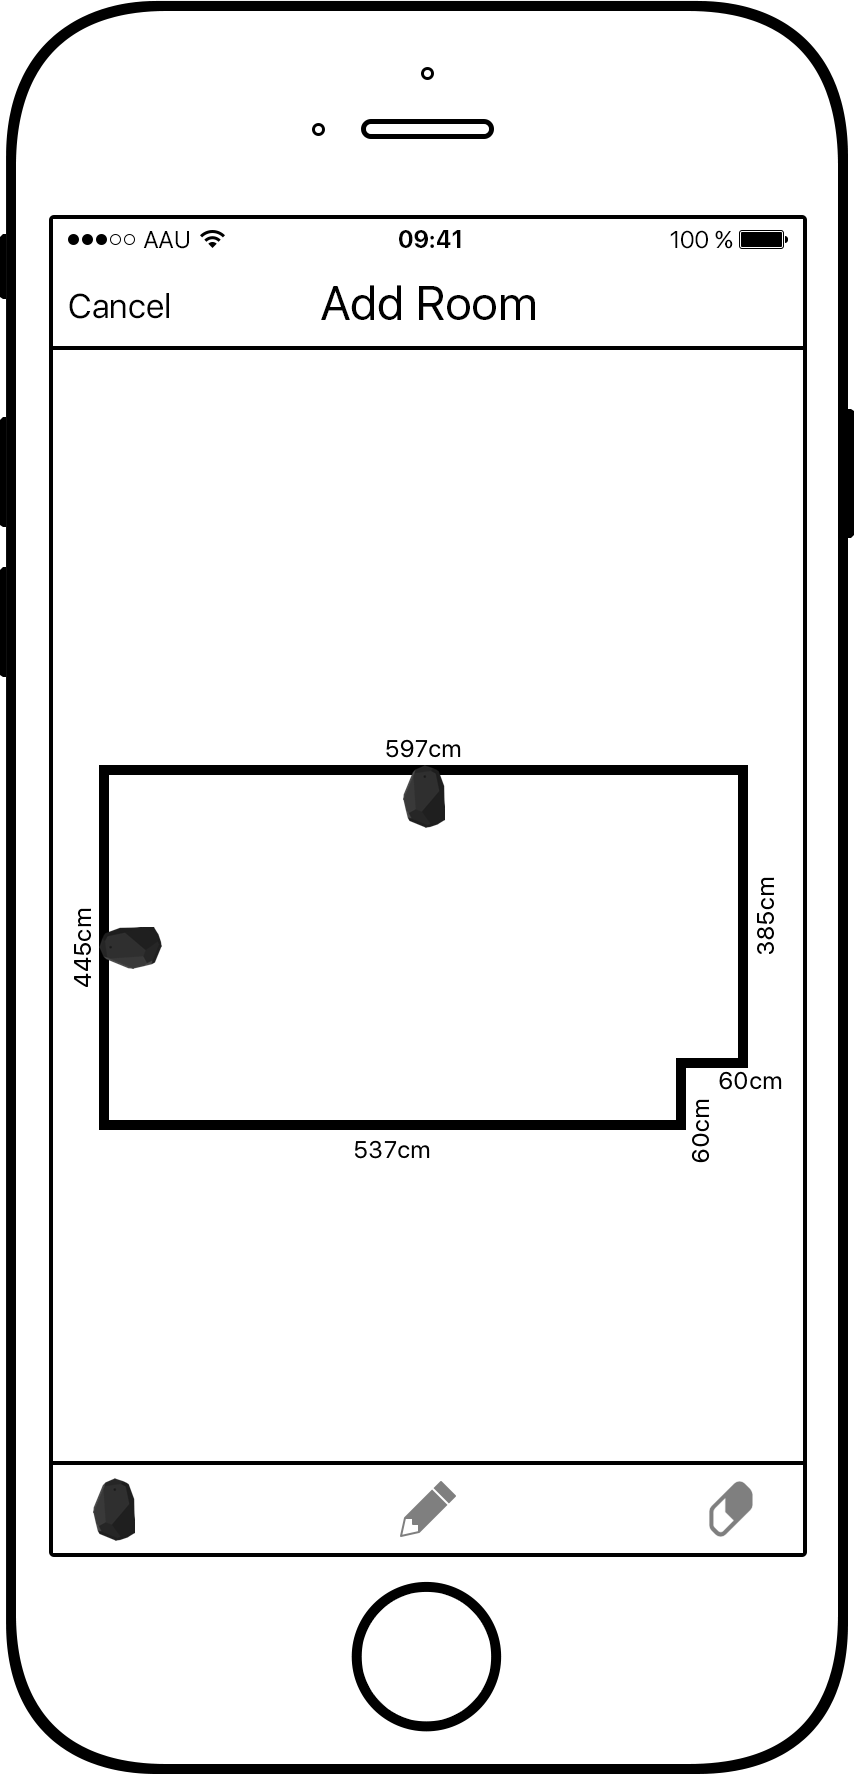
\includegraphics[width=0.3\textwidth]{images/add-room-2}
    }
    \subbottom[Placing actuators]{\label{fig:configuration-location:add-room:actuators}
        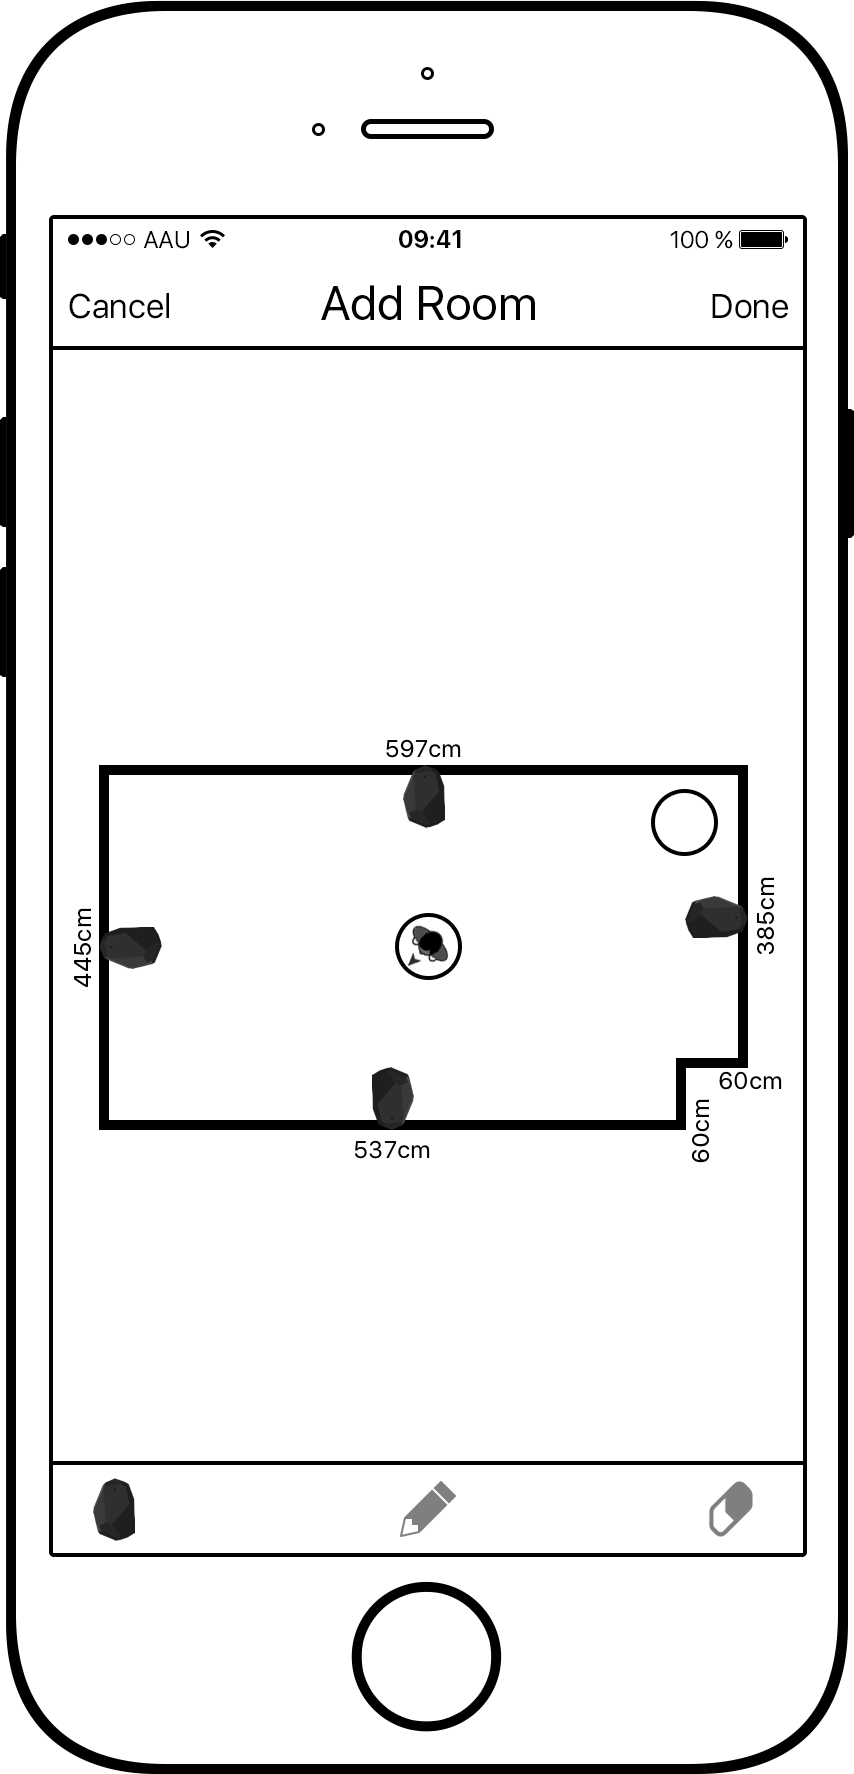
\includegraphics[width=0.3\textwidth]{images/add-room-3}
    }
    \caption{Mock up of software used for configuring locations.}
    \label{fig:configuration-location:add-room}
\end{figure}

%%% Local Variables:
%%% mode: latex
%%% TeX-master: "../../master"
%%% TeX-command-extra-options: "-shell-escape"
%%% End:
